%\documentclass{article}  %%% Pour le type lettre
\documentclass[aps,showpacs,superscriptaddress]{revtex4}%%% Pour le type qui ressemble plus a un article
%%%%%%%%%%%%%%%%%%%%%%%%%%%%%%%%%%%%%%%%
\usepackage[pdftex]{graphicx}   % for figures
\usepackage{epstopdf}
%\usepackage{epsfig}
%draft
\usepackage{dcolumn}
\usepackage{bm}	
\usepackage{ textcomp }
\usepackage{amsmath}			% Mode math\ufffdmatique
\usepackage{amsfonts}			% Polices math\ufffdmatiques
\usepackage{amssymb}			% Symboles math\ufffdmatiques
\usepackage{latexsym}			% Symboles math\ufffdmatiques avanc\ufffds
\usepackage{color}
\usepackage[utf8]{inputenc}
\begin{document}

\renewcommand\thefigure{A\arabic{figure}}  
March 2019,

Dear Editor,

First, we would like to thank the reviewers for their time and their highly valuable comments which have helped improving the clarity and the quality of the manuscript. We acknowledge that a very long time has passed since you sent us back the paper with the reviewers' comments. 
The fact that we took all this time before resubmitting is genuinely due to the fact that the reviewers comments led us to reconsider in depth both the experimental data and our analysis. We went back and took a fresh look at the data, now including data from both conductor and insulator targets, the latter having been previously overlooked by us, made a significant effort in expanding the theoretical description of the instabilities that can take place in the conditions of the experiment and performed as well a very large number of new simulations. 
In short, the new elements brought forward in the paper are as follows:
\begin{itemize}
    \item new data obtained from insulator (PET target) are integrated, and compared to the conductor (Al target) data that were in the previous version of the paper (see Fig. 2)
    \item we have performed an additional, full PIC, simulation in the 2D plane containing the target normal [see Figs. 3(a-b) and Fig. S1]
    \item we have identified that two instabilities can affect the hot electrons: an essentially  collisionless one in the expanding plasmas on both sides of the target, and a resistive one in the target plane. 
    \item we have also expanded our analytical investigations of the instabilities by deriving kinetic and resistive dispersion relations as well as  estimates of    non-linear electric and magnetic field amplitude.
    \item synthetic proton radiographs [see Figs. 4(b-c)] are now performed, using the fields induced by these instabilities, as inferred from the simulations and the analytical investigations, and for two values of the target resistivity, corresponding to the conductor and insulator cases. From these, we clearly see that we obtain two separate sets of structures that are well-consistent with the two sets of structures that are observed in the data. 
    \item finally, we have performed a scan of parameters for the fields (see Fig. S9) and found that the ones that are consistent with the experimental data match well what is expected from the experiment parameters. 
\end{itemize}

As a result, we think we have reached a much better, precise and complete description of the physics at play, which in fact led to the interesting conclusion that we could pinpoint both the  collisionless Weibel-like and the resistive electron filamentation instabilities in these plasmas, which we think should be of significant interest for the community. We believe that at this stage, the revised paper also clarifies most of the points raised by the reviewers. 
This is why we come back now to you, submitting this very substantially revised version of our paper. You will find in what follows out point-by-point answers to the reviewers comments, as well as the corresponding significant changes we made in the article in accordance with their suggestions.

In order to respect the Nature Physics format, a supplemental material which includes details on the analytical calculations, dispersion relation derivation and validation, as well as expanded simulation results (that could not fit in the paper) has been written.

Comments by the referees are numbered and in italic. Our responses are just below.


\section{Reviewer 1 }

\textit{
The manuscript “Experimental evidence of Weibel-type magnetic fluctuations driven by fast electron thermalization in solid targets” by Ruyer et al. analyses the formation of magnetic field structures in the front of solid targets irradiated by intense laser pulses in region far away from the laser spot size. The paper presents experimental evidence regarding these structures and proposes an explanation for the formation of these structures based on numerical simulations (PIC simulations and 2D PIC MHD). The experimental results are very interesting and demonstrate the complex dynamics of B fields in laser-plasma interactions. This is a very timely topic and significant advances should be expected from the laser-plasma experiments that are now addressing these problems.
However, I have some fundamental questions regarding this manuscript that prevent me, at this stage, to recommend its publication in Nature Physics:
}

We thank the reviewer for his/her positive comments regarding  the importance of the magnetic field dynamics in laser plasma experiments, and we hope that our  augmented analysis (in this revised version) of the experimental results sheds a new light on the temporal and spatial scales that characterizes self-generated fields associated with the complex hot electron dynamics.

\begin{enumerate}
%%%%%%%%%%%%%%%%%%%%%%%%%%%%%%%%%%%%%%%%%%
\item  \textit{the authors mention Weibel-type magnetic fluctuations but then the explanation presented in the manuscript indicates that we are in the presence of an instability occurring in a collisional region (actually captured in PIC MHD non electromagnetic simulations), which is a bit puzzling. In my opinion, the title is misleading: if the instability is resistive and collisional in nature how can it be considered Weibel type? This also means that the main motivation for the paper and the introduction need to be revised to properly frame the instability that, according to the authors, is being probed in this experiment; }

We apologize for the lack of clarity of the  previous manuscript.
In fact, triggered by the reviewer’s comments (and the ones of the other reviewers), we have reconsidered in depth both the experimental data and our analysis. We went back and took a fresh look at the data, now including data from both conductor and insulator targets, the latter having been previously overlooked by us, made a significant effort in expanding the theoretical description of the instabilities that can take place in the conditions of the experiment and performed as well a new simulations. 
As a result, we have revised also our analysis of the mechanism that leads to the multiplicity of small-scale circular structures observed on the proton radiographs of the conductor (Al) target, as due to a Weibel-type instability in fact taking place in the collisionless expanding plasma on both sides of the target, normally to it, where favorable conditions for its growth are met.
However, in the conductor target where we observe, on top of the same circular structures, large-scale radial structures, we analyze that the latter originate indeed from resistive filamentation induced within the solid by the hot electrons.

About the latter resistive instability that we analyze, what we aim at is to clarify the role of the background electrons in the  instability taking place in the dense foil.
For this, 
we derived kinetic dispersion relations for Maxwellian hot electrons in a background of cold electrons of current-contribution modeled by the generalized Ohm's law [see Sec. II of the Supplemental material and Fig. 4(e)]. 
The resulting growth rate helps us understand the contribution of the resistive media in stabilizing/destabilizing an anisotropic hot electron distribution. These dispersion relations show, consistently with the vast literature on this subject,  that streaming hot electrons amplify transverse wave fluctuations of wavevector aligned with the cold hot-electron direction. 
The originality of our dispersion relation is in the kinetic treatment of the hot electrons which, although in the non-relativistic limit, allows to assess the influence of a pressure anisotropy or a streaming anisotropy  on the resistive instability. 
The resulting wave is  similar in nature  (non-propagating, magnetic and transverse)  with the wave associated with the Weibel-type instability which is why we previously used Weibel in the description of this instability.  
However,  the main difference is the resistive nature of the media in which the magnetic fields  develop.  We therefore, as suggested by the reviewer, modified the name used to designate the instability and now use resistive (current) filamentation. We also clarified the presentation and the discussions of this instability.

Overall, we think/hope that  we have reached a much better, precise and complete description of the physics at play, which in fact led to the interesting conclusion that we could decouple and compare collisionless Weibel-like and resistive electron filamentation instabilities in these plasmas, which we think should be of significant interest for the community.
We try to make this clear now in Fig. 2  of the main papier which compares experimental radiographs obtained in an  insulator/conductor target and in Fig. 4 which compares synthetic radiographs in high and low resistivity plasmas.

We also, as suggested by the reviewer, modified the title to clarify the findings now highlighted in the revised version of the paper, the new title being:

“Untangling resistive and collisionless electron filamentation instabilities in dense plasmas over large spatiotemporal scales”


%%%%%%%%%%%%%%%%%%%%%%%%%%%%%%%%%%%%%%%%%%
\item \textit{Is the source of the anisotropy the refluxed fast electrons (from the back of the target) or the fast electrons sprayed side ways? For the target thicknesses presented in the paper this cannot be discriminated and I suggest the authors to discuss this point (e.g. by providing experimental evidence/discussing other thicknesses/types of targets); }

We have to distinguish, in our revised analysis, two main types of instabilities affecting the hot electrons: the resistive one, taking place within the foil plane, and the collisionless Weibel-like one, taking place normal to it, in the expanding plasmas on both sides of the target. The first is indeed induced by the electrons sprayed sideways in a resistive medium, while the latter is induced by the electrons participating to the expanding plasma and refluxed along the target normal [as shown in Fig. 3(c) of the main paper].

%Let's define $K_x$, $K_r$ and $K_\theta$, the averaged momentum flux in the $x$ (i.e. normal to the target), radial and poloidal direction respectively that includes the streaming (drift) and temperature contributions.
%Note that while spreading in the target, the resulting  hot electrons distribution has a non-vanishing drift velocity which is aligned with the radial direction.
%
%Rapidly after the initial fast electron spread  taking place during the laser pulse (at $0.5$ ps for $r<200\, \mu$m) and until the end of the PIC-MHD simulation, the $x$, radial and poloidal pressures are  found  to be ordered following $K_x>K_r >K_\theta$  \textcolor{red}{ in most of the simulation domain (see Supplemental material, Fig. 5)} which  indicates that  $K_x/K_\theta>K_r /K_\theta$.
%
%Using the hot electrons parameters extracted from our PIC-MHD simulation, the resistive growth  rate derived  in the ($x,\theta$)-plane, i.e. without particle streaming,  is shown to be larger than the one obtained in the  ($r,\theta$) plane, i.e. with radial streaming.
%This indicates that   the refluxing of electrons that results in $K_x/K_\theta>1$ mainly  drives the field growth compared to the electron spreading in the target plane which results in the particle streaming. 
%This triggers a magnetic modulation of wavevector aligned with the "cold", and therefore poloidal, direction as observed in Fig. 4(a)  of the main paper. 
%\textcolor{red}{ The contribution of the ($x,\theta$) and  ($r,\theta$) anisotropies are now detailed in the Supplemental material (?? Conclusions ??) }

Regarding the target thickness, a comparative study between PET ($10$ $\mu$m thick) and Aluminum  (3 $\mu$m thick)  targets is now included in the revised version of the manuscript. These experimental observations differ mainly due to the target nature (resistivity) and the target thickness is found to have a weak impact, in the $\le 10$  $\mu$m-thickness range.

%%%%%%%%%%%%%%%%%%%%%%%%%%%%%%%%%%%%%%%%%%
\item \textit{From the manuscript, it seems the authors attribute the anisotropy to the fast electron source and the electrons escaping from the focus region. However, is not clear if the origin of the anisotropy is due to the laser-plasma interaction itself (finite spot size simulations could clarify this point) or due to the long temporal evolution of the electron distribution function in the Biermann fields as studied recently by K. Schoeffler et al. PRL and PoP;}

As mentioned above, we now clarify that two different instabilities can affect the electrons: a resistive one taking place in the plane of the target and which is most effective for the insulator target, and a collisionless one taking place in the expanding plasmas on both sides of the target.

A finite spot size laser-plasma fully  PIC simulation has been performed for the aluminum target. 
Because of the very large temporal and spatial scale required in this experiment, this simulation has been performed in 2D dimensions and therefore does not resolve the poloidal direction of the electron spreading (i.e. in the plane of the target). It however allows us to identify and analyze the collisionless instability taking place in the expanding plasmas which are captured by our  2D simulation.
We believe also that this simulation shows that the origin of the anisotropy does not reside in the particular details of the laser-plasma interaction, but rather in the evolution of electrons refluxing in the expanding plasmas.

Indeed, Figs. 1 (d,e,f) of the supplemental material show that  the in-plane hot electron pressure anisotropy is significantly smaller
in the vicinity of the laser-irradiation region ($y<50\, \mu$m) than far from it, where streaming is expected to play a role.

Additionally, our 2D PIC simulation that resolves the laser pulse presents large-scale B-fields   [see Figs. 3(b) and S1(b)] which is typical, in this reduced 2D geometry, of Biermann fields surrounding the plasma plume.
These fields are superimposed to the Weibel-type smaller-scale field fluctuations  and, in the same region of space, the electron phase space is shown to present a double layer which is typical of streaming instability [see. Fig. 3(c)].  

Hence, we are now confident that the hot electron anisotropy that drives the resistive instability  comes from the evolution of the electrons and not from the laser plasma interaction itself nor the Biermann Battery mechanism. 

\textcolor{red}{ The Bierman argument is not included in the supplemental material.  Should we do it and  Ref Shoeffler ?  }

%%%%%%%%%%%%%%%%%%%%%%%%%%%%%%%%%%%%%%%%%%
\item \textit{ Another open question not properly addressed in the manuscript is associated with the region where the B fields are being generated, since proton radiography provides an integrated picture of the fields and the simulations presented/mentioned are 2D transverse or 1D. The manuscript is not clear on how deep into the target these fields are located. }

Again, we have to distinguish the two instabilities that can affect the electrons, and which we try to untangle and analyze in the revised paper: the resistive, in-plane, filamentation, and the collisionless, normal to the target, instability. 
For both,  our analysis is based on the results of the PIC-MHD simulation to infer the characteristics of the E and B fields induced by these two instabilities. The in-plane simulation presented in Fig. 4 has been performed with solid density background   electron as detailed in the methods section. The fields related to the in-plane resistive filamentation are taken as such and used to obtain synthetic proton radiographs [found in Fig. 4(b)]. The resistive magnetic field   obtained in the PIC-MHD simulation is naturally expected to be located over the whole thickness of the dense target.  

As for the E and  B fields induced by the instability in the expanding plasmas, we extract their functional form from the 2D out of plane simulation and from our analytical analysis, relating the electric field to the magnetic pressure as suggested by Refs. [Dieckmann et. al. POP16 (2009); Bret et. al. POP 17 (2010)]. These fields, contained in the expanding plasmas (i.e. within a layer of $48$ microns on one side of the target, see Fig. 3b), are then added to the in-plane fields evoked just above, and the synthetic proton radiographs contained the full fields are shown in Fig. 4(c), both for the low and high resistivity targets. The good agreement we obtained for both cases compared to the experimental data suggests to us that the overall analysis points to the right scenario.

All this is now clarified as follows in the paper:
\begin{itemize}
    \item The expected location of the instabilities is addressed in the manuscript where the description of  Figs. 3(a,b,c) and Fig. 4(a) are made.
    \item Figs. 4(b,c) present our synthetic radiographs.
    \item We describe,  in the Section Methods of the main paper,  the proton-radiography simulation code ILZ and the field description used in order to reconstruct the radiographs.
    \item The influence of the dominant field wavelength on the topology of the observed structures is analyzed in Sec. IV of the Supplemental material. 
\end{itemize}

%%%%%%%%%%%%%%%%%%%%%%%%%%%%%%%%%%%%%%%%%%
\item \textit{To address this point, it would have been quite helpful to have a prediction on the long scale length low density plasma in the front of the target, which for such long time scales is for sure present, and where the Weibel instability (with longer typical wavelengths) can also develop. }

The reviewer is absolutely right, and we thank him/her for this suggestion that pushed us, in order to address this point and also clarify comment number 4, to perform a large 2D fully  PIC laser plasma interaction. In turn, this led to the clarification of the source of the growth of the small-scale, circular structures seen in the proton radiograph and that our revised analysis attributes to the instability growing in this low-density expanding plasma.
The result of this simulation is shown in Figs. 3(a-b). As expected, we can observe that a long scale length low density plasma expands in front of the target after the hot electrons have spread inside the foil.

Because of its reduced geometry, we should note that this simulation does not capture the resistive instability that is expected to occur inside the foil. However, this simulation now allows us to evidenced a Weibel-type instability developing in the expanding plasma and which  was not addressed in the previous version of the paper [See Figs. 3(b,c) of the main paper and Fig. S1 of the supplemental material].
This essentially collisionless Weibel-type instability (or current-filamentation instability) is triggered by the counter stream of the hot electrons and of the  return current electrons in the expanding plasma. 
Such mechanism is consistent with what was reported in two recent publications (Scott et. al. NJP 2017; and Gode et. al. PRL 2017) which  held responsible this mechanism, near the focal spot region, to explain net like structures observed in the TNSA accelerated ions. In both publications, PIC simulations show that the induced magnetic fluctuations  have a dominant wavelength of a few microns.
Figure 3(b) of the main paper shows that this instability can also be driven far from the focal spot ($\ge 100\, \mu$m) after recirculation and dilution  of the hot electrons  inside the foil.

Hence, as already mentioned above, the revised version of the manuscript now addresses two different instabilities:

- The first one is the resistive filamentation which is expected to drive magnetic fields inside the dense part of the foil. The instability was addressed in the previous version of the manuscript and is captured by our in-plane PIC-MHD simulation in reduced 2D geometry [see Fig. 4(a)] and neglecting the influence of the expanding plasma. However it is not captured by the 2D fully PIC laser-plasma simulation.

- The Weibel-type instability    in the expanding plasma is    captured by the fully PIC simulation [Fig. 3(a,b) and Fig. S1]  which resolves the plasma expansion.
 The latter was not addressed in the previous version of the manuscript. Now, a significant part of the revised version of our study is dedicated to its description combining simulation results and analytical estimates to predict the resulting field parameters in realistic geometry.
Note that for this instability,  the dominant magnetic wavelength, which can  be related to the hot electron skin-depth and therefore to the hot electron density, is therefore expected to be much larger for large hot electron dilution. 
This is realized far from the focal spot and at late times, consistently with what can be seen in our experiment.

Note also that a kinetic simulation that would capture both instabilities requires a 3D geometry in order to capture the hot electron dilution in the foil, the laser direction and the plasma expansion direction.  A full-PIC framework is also required along with a simulation domain of  few   $100^3$ $\mu$m$^3$   over at least a picosecond. Such simulation is therefore out of reach of present or near-future super-computers.
Nonetheless, and encouraged by the reviewers suggestion, the insight we now have of the target evolution both in-plane (with the PIC-MHD simulation) and out-of-plane (with the full PIC simulation) gives us access to more complete plasma dynamics than in the previous version of the paper, and now allows us to clarify the roles of the collisionless and resistive filamentation affecting the hot electrons.
We have also reinforced the link with the experimental data by producing synthetic proton radiographs (as detailed in the methods section). These, shown in Figs. 4(b-c), are found to be consistent with the experimental radiographs. This confirms  our revised analysis of the instabilities affecting the hot electrons and that the two instabilities can be disambiguated.  Figures 4(b,c) of  the revised version of the manuscript show that the resistive instability is sensitive to the target nature and results in large radial traces consistent with the observation in PET targets whereas  the collisionless instability  results in the small-scale, circular dark spots  that can be observed in both the PET and aluminum targets.

\end{enumerate}

%%%%%%%%%%%%%%%%%%%%%%%%%%%%%%%%%%%%%%%%%%
%%%%%%%%%%%%%%%%%%%%%%%%%%%%%%%%%%%%%%%%%%
%%%%%%%%%%%%%%%%%%%%%%%%%%%%%%%%%%%%%%%%%%
\section{Reviewer 2}

\textit{This article aims to demonstrate that the structures seen by proton radiography in the experiment performed at the Jupiter Laser Facility's Titan laser at the Lawrence Livermore National Laboratory are magnetic structures produced by a Weibel-type instability.}

\textit{
The interpretation given in this paper in both unconvincing and poorly argued.}
%%%%%%%%%%%%%%%%%%%%%%%%%%%%%%%%%%%%%%%%%%
\begin{enumerate}
\item \textit{From an experimental point of view no real proof is given that the structures detected by the proton radiography technique are magnetic structures (aside from the somewhat simplistic reasoning ``It is used to probe the B-fields developing in target 2 in a "face-on" configuration [33] adapted ........ to minimize the influence of the E-fields that develop along the target normal'.)
Only some shots with an inverted direction of the probe (such as in Cecchetti et al, PoP 16, 043102 (2009) or in Sarri et al, Ref.[43]) could have supported the identification of the magnetic nature of the structures. Otherwise, the ambiguity remains. }


As mentioned in the answers to the comments of reviewer 1, and encouraged by several encouraging suggestions made by all reviewers, we have profoundly revised the paper. In short:
\begin{itemize}
    \item new data obtained from insulator (PET target) are integrated, and compared to the conductor (Al target) data that were in the previous version of the paper (see Fig. 2)
    \item we have performed an additional, full PIC, simulation in the 2D plane containing the target normal [see Figs. 3(a-b) and Fig. S1]
    \item we have identified that two instabilities can affect the hot electrons: an essentially  collisionless one in the expanding plasmas on both sides of the target, and a resistive one in the target plane. 
    \item we have also expanded our analytical investigations of the instabilities by deriving kinetic and resistive dispersion relations as well as  estimates of    non-linear electric and magnetic field amplitude.
    \item synthetic proton radiographs [see Figs. 4(b-c)] are performed, using the fields induced by these instabilities, as inferred from the simulations and the analytical investigations, and for two values of the target resistivity, corresponding to the conductor and insulator cases. From these, we clearly see that we obtain two separate sets of structures that are well-consistent with the two sets of structures that observed in the data. 
    \item finally, we have performed a scan of parameters for the fields (see Fig. S9) and found that the ones that are consistent with the experimental data match well what is expected from the experiment parameters. 
\end{itemize}

Now regarding  reversing the direction of proton probing,
since, as we observe in the data from shot-to-shot, the observed toroids are located at various, \emph{changing positions} on the target (as would be expected from an instability), it would have been impossible anyway to perform any point-by-point comparison between two measurements performed with inverted probing directions; there is indeed no reason the B toroids would be located at the same exact place in the two different shots that we would try to compare.

\textcolor{red}{Present two radiographs from different shots}

Nonetheless, we can speculate the following: Along what is mentioned above, the B-field, resulting in the small-scale circular structures that were solely discussed in the previous version of the paper, is composed of symmetric toroids or ellipsoids of opposite polarities as shown on Fig. 2. 
It is consistent with fields triggered, in the expanding plasmas located on both surfaces of the target, by a thermal-Weibel instability or the current filamentation instability in symmetric-beam configuration. 
The symmetric feature of the B-field (as being present on both sides of the target) implies that inverting the direction of the probe would not give any difference, in terms of the overall pattern on the resulting radiographs.

%%%%%%%%%%%%%%%%%%%%%%%%%%%%%%%%%%%%%%%%%%
\item \textit{Even if we accept, as may well be the case, that the observed structures are magnetic, no mention is made of how the normal currents that are associated with the magnetic ``loops' close at the front of the target. These currents must close somewhere and will generate a more complex magnetic field structure at the front of (outside) the target. This structure can be expected to affect the proton radiography. 2D simulations miss this effect.}

We would first like to point out that the conservation of charge [\emph{i.e.} $\partial_t \rho+\nabla \cdot \mathbf{j}=0$] implies closing of current lines only if we can neglect $\partial_t \rho$, which is  wrong in the region  where the plasma expansion occurs and which is precisely  the region where the fast electrons are expected to bounce during recirculation.
Hence  the current lines  driven inside the dense foil by the resistive instability have no reason to be closed in the expanding plasma.


Note that, in response to various comments from the reviewer,  the generation mechanism of the current field lines and associated magnetic fluctuations inside the dense foil is now also studied by means of a resistive dispersion relation that includes the kinetic response of the hot electrons and resistive return current of the cold target electrons [see Supplemental material and Fig. 3(e) of the main paper]. 

This comment also raises the question of the physics occurring in the expanding plasma,  not captured by our PIC-MHD simulation and poorly addressed in the previous version of the manuscript.
As explained in response to comment 5 of reviewer 1, 
we now present the results of a large fully PIC simulation of the dense aluminum foil irradiated by a high-intensity laser (performed in the plane including the target normal). 
The reduced 2D geometry of this simulation does not  capture the foil poloidal direction and therefore the resistive instability. 
However, these numerical results shed lights on the electron dynamics that occurs in the expanding plasma far from the laser irradiated region ($r \ge 100 \, \mu$m).

As a result, we found that an essentially collisionless instability  is triggered by the counter-stream of the fast particles and the return current electrons  inside the expanding plasma illustrated in Figs. 3(b,c) of the revised manuscript.
A similar mechanism as in Ref. (Scott et. al. NJP 2017; and Gode et. al. PRL 2017)   is expected to occur with the difference that, in our case,  the instability is characterized far from the focal spot ($r > 100 \, \mu$m) and at much later times ($>4$ ps).
We note that the observations of Ref. [Phys. Rev. Lett. Quinn 2012] could also probably be explained by the hot electron recirculation, although  in a wire geometry.
The wavelength (as well as field amplitude) that characterize the instability can be related to the local hot electron skin-depth which,  far from the irradiated region, should be larger, due to hot electron dilution, than the one expected near the focal region (of the order of the critical density). This explains the difference in dominant wavelength between Refs. [Scott et. al. NJP 2017; and Godel et. al. PRL 2017]  and the present experiment (see estimates in the main paper and the calculation details in the supplemental material).

The fields resulting from this instability  are therefore expected to be located in the expanding plasma, a different region than the resistive fields that are expected to be placed inside the dense foil.
Unfortunately, resolving both instabilities in one single simulation requires a  3D geometry (in order to capture the hot electron dilution) full-PIC simulation of laser plasma interaction at solid density over a volume of  few   $100^3$ $\mu$m$^3$   over at least a picosecond and is therefore out of reach of present or near-future super-computers.

However, the revised version of the manuscript now also includes estimates of the wavelength and field amplitude of the field inside the expanding plasma. These estimates are found to compare favorably with our simulations.  Moreover particle tracing simulation (synthetic proton radiographs) that are now performed with the fields extracted from the PIC-MHD simulations indicate that the large radial structures observed in the radiographs of the PET target (not presented in the past version of the manuscript) can be pinpointed to the fields triggered by the in-target resistive instability.
Finally, our estimates of the field amplitude and dominant wavelength of the instability triggered in the expanding plasma are found to be well consistent with the same parameters retrieved (through the synthetic radiographs) dark spots observed in both the PET and the aluminum target. For this, we performed synthetic radiographs while scanning the parameters and found that they match well the data for the parameters expected from simulations and analytical estimates. This is shown in Fig. 4  of the main paper  and in the Supplemental material in Fig. S9.

%%%%%%%%%%%%%%%%%%%%%%%%%%%%%%%%%%%%%%%%%%
\item \textit{In addition in the article no particle tracing simulations are presented from which one could show that the structures are compatible with the deflection from a magnetic field structure and estimate the size and strength of the field. }

The revised version of the manuscript now includes particle tracing simulations, i.e. synthetic radiographs (see Fig. 4), and a quantitative study of the dose modulations on the radiographs of the  fields triggered by both  the resistive and collisionless instability inside the dense foil and in the expanding plasma respectively (see Fig. 2). Such quantitative study is used to infer the values of the field size and strength, both for the magnetic field and non-linear electric field  that are triggered by the instabilities.  These values are found to be consistent with what we expect from the simulations and theory.
As a result of the comparison between the data and the synthetic radiographs (see Fig. 4), we infer that the resistive magnetic fields resulting from our PIC-MHD simulation result in large radial traces consistent with what is observed in the case of the PET target. The estimated fields resulting from the collisionless instability in the expanding plasma results in dark spots are similarly found to be consistent with the structures observed in both the aluminum and the PET target. This is shown in Fig. 4, and also through the scan of the parameters used in the synthetic radiographs that is shown in Fig. S9.

%%%%%%%%%%%%%%%%%%%%%%%%%%%%%%%%%%%%%%%%%%
\item \textit{A filamentation consistent with the development of a Weibel-like instability in the blow-off plasma expanding from the target has been observed by Quinn et al, PRL 108, 135001 (2012). While it would seem fair to cite at least this work along with Ref.[16] where a different approach was used, one may wonder whether the development of filaments oriented along the plasma expansion could produce structures similar to those observed in the proton images of the manuscript. }

We thank the reviewer for his/her insight and this suggestion, which, together with other suggestions, encouraged us to perform the additional full-PIC simulation (in the plane normal to the target surface) that was discussed above.
As also discussed above, we now analyze that the growth of the Weibel-like instability can be, as rightly hinted at by the reviewer, very effective in the plasma expanding from both target surfaces, even far from the laser focal spot. The resulting  E and B fields that we estimated are found to match well the ones which can be inferred from our data, as shown by the scan of parameters used for the synthetic radiographs shown in Fig.4 of the revised paper and Fig. S9 of the supplemental material. Along all the modifications that are now brought to the paper to detail the conditions of the growth of the Weibel-like instability, we also add the reference of Quinn et al. As explained above and in the revised version of the manuscript, we agree with the reviewer that a similar mechanism, with more diluted hot electrons, is responsible of the circular dark spots visible in both the PET and aluminum radiographs. 

%%%%%%%%%%%%%%%%%%%%%%%%%%%%%%%%%%%%%%%%%%
\item \textit{From a theoretical point of view the presentation is rather imprecise and in places confusing, starting from the very title where 'thermalization' of the fast electrons is mentioned while in the text an essentially ballistic mechanism is described (see for example in the abstract ``as they stream radially within the target, their momentum distribution function becomes anisotropic' or later in the text ``assuming a non- relativistic ballistic propagation'). }

We agree with the reviewer that our formulations could have been more precise. The reviewer will see that anyway the paper has been profoundly revised and re-written to incorporate the new material evoked above and provide an hopefully clearer account of the physics at play. Regarding the precise comment, "Thermalization" has now been removed from the text and we believe that the revised version of the manuscript is less confusing regarding the anisotropy of the hot electrons inside the dense foil.
 

%%%%%%%%%%%%%%%%%%%%%%%%%%%%%%%%%%%%%%%%%%
\item \textit{abstract ``laser-generated fast electrons expanding away from the irradiated region.' This expansion would likely create a charge separation and thus tangential electric fields (and possibly return currents and related instabilities). No mention is made of this possible effect, see comment at point b). }

As explained above, an additional 2D full-PIC 2D laser plasma simulation has been performed to clarify the plasma expansion dynamics of the foil during the generation and streaming of the hot electrons. As mentioned rightly by the reviewer, return current streaming instabilities develop in the expanding plasma which description is now detailed in the revised version of the manuscript. As discussed above, the associated fields are held responsible for dark spots visible in both the Aluminum and PET radiographs.

%%%%%%%%%%%%%%%%%%%%%%%%%%%%%%%%%%%%%%%%%%
\item \textit{'whether the typical distance of interaction between particles is, respectively, smaller or larger than the Debye length'. I imagine that distance of interaction (infinite in a Coulomb system) stands for mean free path. }

This sentence concerns the definition  of collective processes in a plasma. This definition can be found in many classical textbooks such as Ref. 1 of our manuscript. 

In a collisionless system, the mean free path tends,  by definition, towards infinity.
However the typical interaction distance between particle, i.e. the scale length that characterizes the process under scrutiny, has a finite value. Otherwise collisionless simulations with kinetic codes (like PIC codes) would be irrelevant. 
A collective process is a process which by definition  has its characteristic lengths larger than the Debye length.
For an homogeneous  and periodic Weibel-unstable system, this distance of interaction is  the dominant magnetic wavelength, i.e. of the order of the unstable population skin depth.

In order to clarify this issue, the introduction has been deeply revised, taking into account the referee's comment.

%%%%%%%%%%%%%%%%%%%%%%%%%%%%%%%%%%%%%%%%%%
\item \textit{references in the Introduction appear to be chosen rather at random simply to fill some generic sentences. A better reasoned selection should be given. Later in the text the authors self-cite Ref.[33] as the observation of fields generated by the "Biermann battery" effect. Such a mechanism was already observed in the above mentioned paper by Cecchetti et al. By the way, it is rather surprising that the omitted references include several co-authors of the present manuscript; what was the bibliographical criterion used by the authors? The manuscript is probably already saturated with self-citations but the most relevant ones might have been omitted. }

We would first like to underline that the paper of Cecchetti et al has been the result of another collaborative work from our group. Thus, the paper by Cecchetti et al. is of course not at all unknown to us since this was the first time our group performed B-field probing, and it was the first time this was done using TNSA, broadband accelerated protons (in contrast with the work performed by Li et al around the same time using monochromatic protons produced by implosions at LLE). We rather cited the paper of Albertazzi et al. because: i) it pertains to probing of B-field generated by high-intensity, short-pulse lasers, when our previous work (reported in Cecchetti et al) was aiming at probing B field generated by long pulse lasers, and ii) the data we analyze in the present paper has been obtained using the setup detailed in Albertazzi et al. These are the very reasons for citing that work, and not randomness. Note finally that the paper of Cecchetti et al. can be found as a reference in the paper of Albertazzi et al. So, we now precise “and refs therein”. 

We would then like to underline that although there are indeed several citations from works performed by our collaborative group, these are a minority of all the cited papers. Respectively 76\% and   80\% of the citations in the previous and revised version of the manuscript are from other works. If there are some self-citations, this is due to the fact that we have been collectively active in characterizing laser-acceleration of high-energy protons, and in pioneering their use as probes of electric and magnetic fields. 

Note that the number of references are limited to 50 in the Nature Physics format, hence we can’t cite all the papers that would be good to cite to be thorough.

As mentioned above, we also deeply revised the introduction.

%%%%%%%%%%%%%%%%%%%%%%%%%%%%%%%%%%%%%%%%%%
\item \textit{It is also surprising, looking at previous work, that this time no effort has been made to perform particle tracing simulations. }

We apologize for the lack of particle tracing in the previous version of the manuscript. As mentioned above, these are now included, being part of a large effort from our part to expand our analysis.
We hope that with the revised version of the paper, the reviewer will find a much deeper analysis including comparative particle-tracing simulation for different targets  with  various self-generated field addressed in the study. 
These simulations are illustrated in Figs. 4(b,c) and details are presented in the section method and in the supplemental material.

%%%%%%%%%%%%%%%%%%%%%%%%%%%%%%%%%%%%%%%%%%
\item \textit{strictly speaking pressure anisotropy, not momentum anisotropy is at the basis of the Weibel instability. Momentum anisotropy may simply imply fluid streaming in a given direction, which would have nothing to do with the Weibel instability. This is not simply semantics since later the definition of $K_r$ seems to suffer from this misunderstanding as it corresponds, at least in part, simply to ordered (i.e.``fluid') radial motion of the hot electrons. }

To illustrate the difference between the thermal Weibel (Weibel, PRL 1959) and current filamentation (Fried et. al. PF 1959) instability, let's examine the case of a plasma composed of two counter streaming drifting multi-Maxwellian plasma with infinite-mass ions.
We now introduce the 2D electron normalized  distribution functions as follows:
 \begin{equation}
f_{ \pm}(v_x, v_y)  = \frac{ m_e }{2 \pi \sqrt{  T_x T_y  } }\exp\left( -\frac{ m_e (v_x \pm v_0)^2 }{ 2T_x }  -  \frac{ m_e v_y^2 }{ 2 T_y }\right) \, .
 \end{equation}
The associated kinetic dispersion relation of wavevector aligned with the $y$ direction has been solved in Ref.  (Davidson PF 1972) without drifts ($v_0=0$). The dispersion relation can be easily generalized to the above distribution function (with a drift)
following Ref. (POP Ruyer et. al. 2012),  giving
 \begin{equation}
 \omega^2 -k_y^2c^2 -  \omega_{pe}\left( 
1 -  \frac{ m_e v_0^2  + T_x }{ T_y }  ( 1 +\xi_\pm \mathrm{ Z }(\xi_\pm)  ) 
\right) =0 \, ,
 \end{equation}
where $ \mathrm{ Z }$ is the plasma dispersion function, its argument is $\xi_\pm =\sqrt{  m_e/2 T_y  }   \omega/k_y$, and 
$\omega_{pe}$ is the total electron plasma frequency. As is well known, the above equation has non-propagating unstable solution ($\mathrm{Real}(\omega)=0$ and $\mathrm{Imag}(\omega)>0$) when $m_e v_0^2  + T_x > T_y$.
This can be achieved in a non-streaming system (pressure anisotropy), giving $T_x > T_y$ as for the thermal Weibel instability. 
Or it can be obtained in the limit $m_e v_0^2  \gg T_x$ so that, the instability condition becomes  $m_e v_0^2  > T_y$ which is the purely streaming limit, i.e.  the current filamentation instability.
However, these are two limits of the same dispersion relation. Therefore we cannot agree with the sentence: " \textit{Momentum anisotropy may simply imply fluid streaming in a given direction, which would have nothing to do with the Weibel instability. This is not simply semantics...}". 
Although not identical, these two instabilities are   close as they both   have the same unstable loop that amplifies the transverse wave.

However, in order to be accurate, care has been taken to clarify the role of streaming or pressure anisotropy  in our description of the two different instabilities now described in the manuscript.
The supplemental material now includes the kinetic dispersion relation of the resistive filamentation indicating that pressure anisotropy is dominant in triggering the magnetic fields regarding the resistive instability that takes place in the dense part of the target, a few picoseconds after the laser pulse.
Regarding the  return current instability taking place in the expanding plasma, the streaming of particles is probably the dominant process as two distinct beams are present in the electron phase space of the expanding plasma, Fig. 3(c).

%%%%%%%%%%%%%%%%%%%%%%%%%%%%%%%%%%%%%%%%%%
\item \textit{The B2 pulse is oblique incident but I could not find the value of the angle. Fig 2 seems to show that, despite the angle of incidence, the detected structures are symmetrically distributed around the central spot, as expected in the case of thermal expansion, but irrespectively of the directionality of the pulse. This does not seem so easy to understand for the trapped-reflected electrons that contribute to the large (constant) value of $K_z$ ('Those electrons injected at large angles into the target will drift far away from the irradiated region'). This directionality is also suggested by Fig.2. }

We thank the reviewer for attracting our attention on this point since, as developed below, it supports our analysis of the dynamics at play here.

First, we apologize for the lack of precision on this point: the laser B2 is incident on target with an angle of 31$^O$, in the horizontal plane, compared to the target normal.
This is now stated in the Methods section.

\begin{figure}[tbh!]
\centerline{
\begin{tabular}{c}
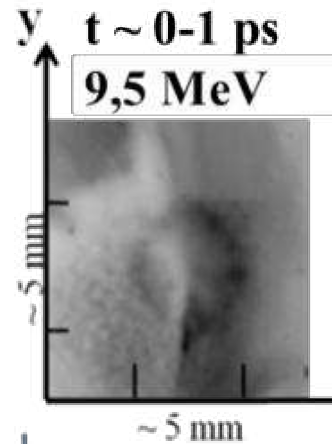
\includegraphics[scale=0.5]{RCF_1ps_Al.png}\\
\end{tabular}}
\caption{\label{fig:xp} Early time proton radiograph for an Aluminum $3\, \mu$m-thick foil. The laser pulse comes from the top right and is focused at the central region of the radiograph.
}
\end{figure}
Very early time experimental radiographs obtained for Aluminum targets
does suggest a directionality of dark spot-like structures in accordance with the laser orientation. This radiograph, illustrated in Fig. \ref{fig:xp} of this document and which can be found in Ref. (Phd Albertazzi) and Fig. 2(a) of Albertazzi et al., was not included in the previous version of the manuscript because of the imprecision of the associated probing time (around the time of irradiation, with a precision of 1 ps).   
However, it clearly shows, as discussed by the referee, that a preferential direction consistent with the laser direction is given to the early time development of these structures.
Finally at the final time of our large scale PIC-MHD simulation ($1.4$ ps), a clear preferential direction is as well observed  on the self-generated field  in the expanded plasma (see Figs. S1a,b of the supplemental material where magnetic fluctuation can be seen for $y>0$), consistently with Fig. \ref{fig:xp}. At 1.4 ps, our laser plasma simulation shows  hot electrons located in the domain opposite to the laser orientation ($y<0$), although their density is smaller than for $y>0$ (see Fig. S3a). At later time ($t>1$ ps), after the end of the main laser drive, we expect that no preferential direction is given to the  hot electrons and we therefore expect their recirculation to take place inside the foil, independently of the laser orientation.

Three sentences are now included in the manuscript (second page, second column, second paragraph of the main paper): "Moreover, they are mainly located at the left-hand side ...".

%%%%%%%%%%%%%%%%%%%%%%%%%%%%%%%%%%%%%%%%%%
\item \textit{The wave number dependences of the Filamentation and of the Weibel instability growth rates are very similar (see e.g. the vast literature on this subject in the '90s ) in the long wavelength limit which is the one relevant for the proton radiography. Thus the sentence ``One possible origin for the observed loop-type structures could be the development of the electron current filamentation instability, which is known to generate small-scale magnetic fluctuations in the dense plasma close to the laser focal spot [10, 11]. However, the typical scale of these B-fields is of the order of the bulk electron plasma ,,,,,. Moreover, the resolution of the diagnostic being limited by the proton source size of a few microns [38], such small scale B-fields cannot be detected, thus invalidating this scenario.' is both unnecessary (it is very difficult to distinguish unambiguously between the two instabilities in the presence of streaming particles) and incorrect.} 

We believe there was a misunderstanding here. We meant that, 
as the source size of the TNSA protons is of a few microns, the radiography cannot probe wavelength smaller than a few microns.  
We do not aim at discriminating between the Weibel and current filamentation but rather to highlight that the radiograph diagnostic of our experiment cannot detect the sub-micron magnetic wavelength that are expected in the vicinity of the irradiated region.

We  agree with the referee on the unnecessary feature of this paragraph;  it has been  removed from the  paper.

%%%%%%%%%%%%%%%%%%%%%%%%%%%%%%%%%%%%%%%%%%
\item \textit{Figure 3 is difficult to read (too many similar colours). In addition it is absurd to plot the ballistic estimate for $K_r$ at time $ t = 0.34 ps$ in a region $r > say 120$ where there are no hot electrons yet. }

This curve has been removed from the deeply revised version of the manuscript and care has been taken to apply this comment to the new figures present in the manuscript.

%%%%%%%%%%%%%%%%%%%%%%%%%%%%%%%%%%%%%%%%%%
\item \textit{What is the mechanism that reduces $K_r$ over time? no mention is made in the article. Why is $K_r$ interpreted as a temperature (I would understand it in part by referring to the overall cold and hot population at a given position) and not simply as ordered streaming energy? This is not the case for $K_z$ which is closer to a temperature because of the multiple reflections along z inside the target.}

As defined in the previous version in the manuscript, Kr was the averaged radial momentum flux. For a Maxwellian distribution, it reads $K_r = T_r +m v_r^2$ and is  the sum of the temperature and the streaming contribution.
In the ballistic estimates $K_r  \sim m_e r^2/t^2$ we neglected  $T_r$ in front of $m v_r^2$ because the electron phase space suggested that it was a fair approximation. The decrease of $K_r$ is due, in first approximation, to ballistic effects : the particle that travels the distance r in a time t without energy exchange along its path (i.e. ballistic approximation) has necessarily a velocity given by $r/t$. 
However, these estimates have been removed from the manuscript.

%%%%%%%%%%%%%%%%%%%%%%%%%%%%%%%%%%%%%%%%%%
\item \textit{The sentence ``At later times, we expect the magnetic structures observed in Fig. 4 to become increasingly circular, i.e., to evolve closer to the behavior witnessed in the radiographs of Fig. 2. ... Therefore, we expect the initial hierarchy between $K_r $and $K_\theta$ to reverse' appears simply a way to make theory and data fit. Certainly the reason given is insufficiently motivated, in particular in connection with the behavior at late times of $K_\theta$. Indeed, it is not straightforward (to say the least) to infer any similarity between the simulation result shown in Fig.4 and the experimental observations. }

A deep revision of our study has been made in order to address this fair comment. As detailed above, in addition to the PIC-MHD simulation already presented in the manuscript, we have performed for the revised version of the paper a large scale laser-plasma interaction full PIC simulation in reduced 2D geometry that demonstrates that a return current streaming instability can take place in the plasma expansion, at least 100 microns away from the focal spot.

As explained in the manuscript, we now believe that the fields generated in the expanding plasma are responsible of the dark spot-like structure visible in the PET and Al   radiographs and that the resistive instability triggered in the dense plasma, sensitive to the target resistivity, is responsible for the large radial traces observed for the PET target only. Simulations of particle tracing (i.e. synthetic radiographs) have been performed to support our scenario. We believe that we have now a much stronger and clearer connection between the simulations, theory and experimental data, their consistency supporting compellingly the scenario outlined in the paper and discussed above.

%%%%%%%%%%%%%%%%%%%%%%%%%%%%%%%%%%%%%%%%%%
\item \textit{Eq 1: the magnetic Lorentz force in the generalized Ohm's law, if written in terms of the current density, needs the electron charge in the denominator, not simply the electron density. }

We thank the reviewer for having spotted this, the formula has been corrected.

%%%%%%%%%%%%%%%%%%%%%%%%%%%%%%%%%%%%%%%%%%
\item \textit{Small point: strange repeated mistake in the initials of the authors of Ref.[19] }

The reference has been corrected

\end{enumerate}

%%%%%%%%%%%%%%%%%%%%%%%%%%%%%%%%%%%%%%%%%%
%%%%%%%%%%%%%%%%%%%%%%%%%%%%%%%%%%%%%%%%%%
%%%%%%%%%%%%%%%%%%%%%%%%%%%%%%%%%%%%%%%%%%
\section{Reviewer 3 }
\textit{
In this work, magnetic fluctuations of the Weibel type are observed in an expanding plasma heated by a short pulse laser focused to small scale and high intensity. This creates an expanding relativistic electron population, partly confined by electrostatic sheath fields. The authors observe filamentary magnetic field structures using an established proton-radiography technique. The magnetic field structures consist of a number of normal-directed currents of both signs giving rise to magnetic field loops. The filamentary structures well-match to a qualitative picture for Weibel-type of fluctuation. To help interpret these observations, some interpretive simulations have been done; these appear to me to not strong agreement with the observations; these indicate possible interpretation issues (to be discussed below).}

\textit{
On the broad applicability of the results, the results are interesting, as there is great interest in the role of Weibel instability in collisionless plasmas, and there have not been a large number of observations driven by electron anisotropy. The results will likely be important for understanding laser-plasma and laser-solid interactions in certain regimes. The authors provide a pretty good background discussion and set of references. At the same time, the actual experimental setup, where the longitudinal confinement of the electrons is apparently important, seems to be rather fortuitous. This specialized geometry (longitudinal confinement) does not readily map to many particular problem (for example shocks), or to the beam-Weibel instability of great lore for fast-beam slowing down. Overall, I support publishing this paper in a high-profile journal such as NPhys.}

We thank the reviewer for his/her positive comments regarding the interest of our work. As detailed in the answers to reviewers 1 and 2 above, we have, encouraged by all reviewers’ suggestions, revised in depth our work.
Briefly, we have brought the following major changes to the paper:
\begin{itemize}
    \item new data obtained from insulator (PET target) are integrated, and compared to the conductor (Al target) data that were in the previous version of the paper (see Fig. 2)
    \item we have performed an additional, full PIC, simulation in the 2D plane containing the target normal [see Figs. 3(a-b) and Fig. S1]
    \item we have identified that two instabilities can affect the hot electrons: an essentially  collisionless one in the expanding plasmas on both sides of the target, and a resistive one in the target plane. 
    \item we have also expanded our analytical investigations of the instabilities by deriving kinetic and resistive dispersion relations as well as  estimates of    non-linear electric and magnetic field amplitude.
    \item synthetic proton radiographs [see Figs. 4(b-c)] are performed, using the fields induced by these instabilities, as inferred from the simulations and the analytical investigations, and for two values of the target resistivity, corresponding to the conductor and insulator cases. From these, we clearly see that we obtain two separate sets of structures that are well-consistent with the two sets of structures that observed in the data. 
    \item finally, we have performed a scan of parameters for the fields (see Fig. S9) and found that the ones that are consistent with the experimental data match well what is expected from the experiment parameters. 
\end{itemize}

As a result, we believe that we have now a much stronger and clearer connection between the simulations, theory and experimental data, their consistency supporting compellingly the scenario outlined in the paper and outlined just above.\\


\textit{
Now, I also have a few of questions on the interpretation which should be addressed, and for which I would be happy to read the authors responses and revisions.}

\textit{
The underlying picture, that the anisotropy drive for the instability comes from the cooling of a transversely expanding electron cloud confined to the target, is certainly a plausible explanation. However, the connection of this picture to the experiment results are not detailed or explained enough. At least, I remain with significant questions -}

\begin{enumerate}
%%%%%%%%%%%%%%%%%%%%%%%%%%%%%%%%%%%%%%%%%%
\item \textit{Most fundamentally, I did not find explanation 100-$\mu$m wavelength of the instability; this is very fundamental to the interpretation and should be provided. The dispersion relation for Weibel is well-known, of course, the question is to identify the relevant plasma "players" and source and magnitude of anisotropy. In this case, I think the authors did not explain the role of the background solid density plasma - should this not do a very good job screening fluctuations - which indeed are at much larger than the electron skin-depth scale? The authors indeed correctly point out that the wavelengths observed are much larger than many of the standard beam-driven Weibel predictions, which are of order the electron skin depth. This must be better explained. }

Aiming at clarifying the role of the background plasma on the kinetic instability,
we derived the kinetic dispersion relations for Maxwellian hot electrons in a background of cold electrons of current-contribution modeled by the generalized Ohms low. 
The resulting growth rate obtained to third order in $\Gamma/k v_{th,y}$ help us understand the contribution of the resistive media in stabilizing/destabilizing an anisotropic hot electron distribution. 
The calculation details are presented in the supplemental material where we show that the
resistive media significantly decreases the instability growth rate compared to a non-resistive case (without resistive electrons).
As expected, the growth rate increases when increasing the background resistivity for anisotropic enough hot electrons as now shown in Fig. 3(e) of the main paper.
These results represent one of the key results used to  revise the manuscript,  shedding light on the role of the dense plasma in the instability addressed.

As suggested by the reviewer,   the large wavelength observed in our radiographs is one of the surprising results of the  experiment. As mentioned above, we have now performed an additional full-PIC simulation (in the plane normal to the target), as well as simulated synthetic radiographs that allow us now to better localize the source of the Weibel-like instability as originating from the plasma expanding from both target surface. In particular, we show in Figs. 4(b,c) that the resulting synthetic radiographs are well consistent with the experimental observations. 

%%%%%%%%%%%%%%%%%%%%%%%%%%%%%%%%%%%%%%%%%%
\item \textit{Possibly related, the simulations results offered in Fig. 4 appears to me to be in significant disagreement with the data; the fluctuations appear to have poloidal wavelengths of order $\sim 5 \mu$m (and not really the 30 $\mu$m quoted on page 8... at least by my eye on the figure), whereas they are of order 100 $\mu$m in the radiograph. Since the wavelengths of the Weibel often scale with the skin depth of the interacting plasmas; this possibly indicates a very significant difference in the density where the interaction is occurring, possibly indicating the overall picture of where and how the interaction occurs, as presented in the paper is not correct. }

The reviewer is right in underlining the difficulty with our previous analysis. As mentioned above, we have now gone several steps further, by performing a  large fully PIC simulation of laser plasma interaction. Now included in the manuscript, it evidences magnetic fluctuations triggered in the expanding plasma during the recirculation of the hot electrons [see Figs. 3(a,b,c)]. This collisionless Weibel-type instability presents a dominant magnetic wavelength of the order of $\sim 10 \, \mu$m.
We should note that the reduced 2D geometry of our numerical results under estimates the hot electrons dilution during their stream in the foil targets. 
By mean of a simple analytical modeling of the hot electron dilution, validated by comparison with our PIC-MHD simulations [see Fig. 3(d) and supplemental material], and by also performing synthetic radiographs, we  estimate the  dominant magnetic wavelength in realistic geometry and the overall electric and magnetic field topology to be consistent with the one extracted from the dark spot-like structures of the Aluminum  and PET targets due to the dilution of the hot electrons inside the foil.
Indeed, the dark spot-like structures are observed $t_{xp}   = 8$ ps   after the main laser drive, hundreds of  microns from the irradiated region.
Since the hot electron deposition region extracted from our fully PIC simulation is of the order of $R_0\sim 20\, \mu$m, 
a dilution factor of at least $t_{xp} v_h / R_0 \sim 120$ (for a hot electron velocity $v_h$ of the order of  the light speed) is to be expected. Hence, we estimate a hot electron skin-depth at least  an order of magnitude larger in the experiment than in the 2D full PIC simulation,  and therefore a dominant magnetic wavelength consistent with our observations.
Care has been taken to verify that the corresponding growth time is, after hot electron dilution, sill consistent with the observations.

Overall, we now conclude that the large radial structures seen in our first simulations were not consistent with the one observed for the Aluminum foil, but far more consistent with the radiographs resulting from  PET targets and performed in the same experimental campaign, although  not included in the previous version of the manuscript. Based on all this material, we also conclude that the origin of the small-scale circular structures rather originates from the filamentation in the expanding plasmas from both target surfaces. 
As now explained in the main paper,  our resistive dispersion relations resolved  with the hot electrons parameters extracted from our PIC-MHD simulation suggest that the system is more unstable as the resistivity increases,  i.e. for PET targets compared to aluminum targets. Hence, the large radial structures induced by the resistive filamentation are expected to be more detectable for the PET than for the Al targets, as observed in the experiment.

Regarding the field topology, 
Ref. (Scott et. al. NJP 2017; and Godel et. al. PRL 2017) shows that the return current instability amplifies roughly circular field lines in the expanded plasma, although these observations are made in the vicinity of the irradiated region at early times.


%%%%%%%%%%%%%%%%%%%%%%%%%%%%%%%%%%%%%%%%%%
\item \textit{Another related point to the dispersion relation - Figure 3 presents the evolution of the momentum flux of hot electrons. But, whether this is the correct quantity to analyze depends on what is driving the instability - again is it driven purely by the anisotropy of the hot electrons (which is not exactly equal to the ratio of the quantities plotted), or interaction of the hot electrons and solid plasma (requiring the effective anisotropy of the whole distribution including hot and cold)? This would all be much better clarified if the authors present and solve the relevant dispersion relations (would be perfect to include these in supplementary material). }

  The reviewer is right. The fully electromagnetic resistive dispersion relation has been solved and is now included in a supplementary material. It shows that the growth rate is reduced compared to the collisionless case of a hot and cold electron streaming instability. The wavelength maximizing the  growth rate  also shifts to larger values.  

As explained above and suggested by our reviewers, these dispersion relations are now included in the paper and in the supplemental material.

\item \textit{
I view this main criticism as largely all connected together; I encourage the authors to provide some more details on the interpretation; surely they have thought these issues through.}

All comments suggestions and positive criticism  were carefully analyzed and the  appropriated corrections were   made in the study, leading to more analytical modeling, a supplementary large scale simulation of laser plasma interaction, and additional  PIC-MHD simulations varying the hot electron initial parameters.

During the deep revision of our manuscript, an effort has been made to take into account the different comments and their relative connection  in a self-consistent way. As a result all figures, except Fig. 1, were modified and the major part of the manuscript has been rewritten. We believe that a much clearer and consistent picture has thus emerged, allowing this work to advance our picture and understanding of the instabilities affecting hot electrons in various regimes.




%%%%%%%%%%%%%%%%%%%%%%%%%%%%%%%%%%%%%%%%%%
\item \textit{
In conclusion, I think the authors have made a nice set of measurements which certainly qualitatively looks like it could be a Weibel in a novel regime; however I am struggling to be convinced of the interpretation. I look forward to additional thoughts from the authors.}

We thank the reviewer for his kind comment and hope that his/her requests are satisfied by the deeply revised version of our study.


\end{enumerate}




\end{document}